\documentclass[
8pt, % Set the default font size, options include: 8pt, 9pt, 10pt, 11pt, 12pt, 14pt, 17pt, 20pt
%t, % Uncomment to vertically align all slide content to the top of the slide, rather than the default centered
%aspectratio=169, % Uncomment to set the aspect ratio to a 16:9 ratio which matches the aspect ratio of 1080p and 4K screens and projectors
]{beamer}

\graphicspath{{Images/}{./}}

\usepackage{booktabs}
\usepackage{ctex}

\usetheme{Madrid}

\usefonttheme{default}

\usepackage{palatino}
\usepackage[default]{opensans}
\usepackage{makecell}
\usepackage{listings}
\def\pgfsysdriver{pgfsys -dvipdfmx.def}
\usepackage{tikz}
\usetikzlibrary{positioning}

\useinnertheme{circles}

\lstset{
    basicstyle      = \small\sffamily,
    keywordstyle    = \color{blue},
    commentstyle    = \color{red},
    stringstyle     = \ttfamily,
    flexiblecolumns,
    numbers         = left,
    showspaces      = false,
    numberstyle     = \tiny,
    captionpos      = b,
    showstringspaces= false
}

\lstdefinestyle{Assembler}{
    language    = [x86masm]Assembler,
    basicstyle  = \small\sffamily,
    numbers=left,
    numberstyle=\tiny,
    frame=tb,
    tabsize=4,
    columns=fixed,
    showstringspaces=false,
    showtabs=false,
    keepspaces,
    commentstyle=\color{red},
    keywordstyle=\color{blue}
}

%----------------------------------------------------------------------------------------
%	PRESENTATION INFORMATION
%----------------------------------------------------------------------------------------
\title{参与研究安全操作系统的初步想法}
\institute[Massclouds]{\large 乾云科技}
%----------------------------------------------------------------------------------------

\begin{document}
	\renewcommand\arraystretch{2}

	%----------------------------------------------------------------------------------------
	%	TITLE SLIDE
	%----------------------------------------------------------------------------------------
	\begin{frame}
		\titlepage
	\end{frame}

	%----------------------------------------------------------------------------------------
	%	OBJECTIVE
	%----------------------------------------------------------------------------------------
	\begin{frame}
		\frametitle{目标}
		{\large 从zCore起步,参与安全操作系统的研究工作:}
		\begin{itemize}
			\item {\large 发展一个面向AIoT领域的安全操作系统,以RISCV为主要目标体系结构,向上提供与Zircon保持同步的系统调用接口 以及 与Linux kernel保持兼容的系统调用接口。}
			\item {\large 以Rust-lang为主要的实现语言,架构上参照Zircon的整体架构设计, 实现参考Linux kernel(arch/riscv), Redox等。}
			\item {\large 通过开源社区的方式组织研究和开发,建立各层面开发者参与协作的通道,建立应用层面使用者的反馈通道。}
		\end{itemize}
		{\large 下面就目前进行的准备工作和对将来工作的设想做一个汇报:}
	\end{frame}

	%----------------------------------------------------------------------------------------
	%	TABLE OF CONTENTS SLIDE
	%----------------------------------------------------------------------------------------
	\begin{frame}
		\frametitle{纲要}
		\tableofcontents
	\end{frame}

	%----------------------------------------------------------------------------------------
	%	PRESENTATION BODY SLIDES
	%----------------------------------------------------------------------------------------
	\section{zCore学习过程和疑问}

	\begin{frame}
		\begin{center}
			{\LARGE 对zCore的学习过程及疑问\\}
			\bigskip\bigskip
			{\large 仅针对BareMetal RISCV平台 - 9月15日版本}
		\end{center}
	\end{frame}

	\subsection{引导阶段}

	\begin{frame}
		\frametitle{1 入口\_start}
		\begin{enumerate}
			\item 通过select\_stack为primary hart查找和配置内核栈,为函数调用作准备
			\begin{block}{}
			建议这里不必按照固定的最大值(MAX\_HART\_NUM)为所有的harts预分配页。
            此时还不知道Harts的总数。可以只为primary hart在bss中预分配栈,
            等primary hart初始化过程中确定harts数量之后,再按需分配。
            启动secondary harts可以改一下,把它们的启动时机推后,具体想法后面会提到。
			\end{block}
			\item 进入primary hart的启动函数primary\_rust\_main
			\item 清零BSS段
			\item 初始化页表,为切换到虚拟空间作准备(见2)
			\item 检查设备树dtb有效性
			\item 启动secondary harts(见3)
			\item 进入下阶段primary初始化
		\end{enumerate}
	\end{frame}

	\begin{frame}
		\frametitle{2 启动阶段页表设置boot\_page\_table}
		\begin{enumerate}
			\item 设置物理地址与虚拟地址恒等的跳板页
			\item 从虚存开始地址映射物理空间的前128G
			\item 基于SV39模式启用mmu
			\begin{block}{}
				目前zCore是固定采用sv39的模式。
                可以借鉴Linux kernel的方式, 通过写后读satp轮流尝试sv57,sv48,
                自动检测并启用所在硬件平台支持的最大模式。
			\end{block}
			\item 调整栈寄存器sp和返回地址寄存器ra, 完成从物理空间到虚拟空间转换
			\item 设置状态寄存器, 从此允许kernel访问User页面
			\begin{block}{}
				建议采取保守策略, 默认情况下始终不开, 即默认不允许内核直接访问用户页面。
                仅在kernel/user之间执行内存拷贝或设置的时候, 再临时打开, 操作完后随即关闭。
			\end{block}
		\end{enumerate}
	\end{frame}

	\begin{frame}
		\frametitle{3 启动Secondary Harts}
		\begin{enumerate}
			\item 检查sbi是否支持HSM扩展,不支持则退化为单核系统
			\begin{block}{}
				HSM是OpenSBIv0.7之后才支持,可以参考Linux kernel for riscv的处理方式:\\
				(1)这里不检查HSM的支持。\\
				(2)把那个Atomic全局变量STARTED提前到\_start入口位置,用它保证只有一个Hart能通过,
                其它在STARTED变量spin等待。那个唯一能通过的就是Primary Hart。\\
				(3)Primary Hart启动各secondary harts时, 如支持HSM, 就如当前的办法用SBI唤醒;
                不支持的, 打开STARTED的封锁, 让secondary hart开始自己的初始化过程。
			\end{block}
			\item 遍历设备树文件dtb,发现primary之外所有的hart,通过SBI启动它们,执行secondary的启动流程(见4)。
			\begin{block}{}
				感觉这里就启动secondary harts有点早了,一是这里需要单独处理dtb,其它几处还有单独处理dtb的地方,代码有点分散;二是启动了后面也没有真正运行,还是要等primary的信号。
				建议由Primary Hart在一处统一处理dtb,生成各种管理结构,包括Harts对象数组,然后为所有secondary harts准备好栈,再kick它们。
			\end{block}
		\end{enumerate}
	\end{frame}

	\begin{frame}
		\frametitle{4 Secondary Hart的启动流程}
		\begin{enumerate}
			\item 设置栈:zCore直接用hartid这个硬件ID作为CPU的编号,用它来对应包括系统栈在内的各种CPU专属资源。
			\begin{block}{}
				直接利用hartid作为CPU编号有点问题。
				按照Riscv规范【The RISC-V Instruction Set Manual - Volume II: Privileged Architecture】3.1.5节:
				至少有一个HART的hartid是零,但并不要求所有hartid是连续的。实现策略由厂商自行决定。
				由于不能保证hartid是从零开始的连续数值区间,所以当索引不合适。建议按照通常做法,维护一个CPU数组,CPU在数组的位置即逻辑ID作为CPU资源的索引。
			\end{block}
			\item zCore占用TP寄存器来维持hartid。
			\begin{block}{}
				在系统中, Hart的硬件ID不连续不能作索引, 所以不常用。
                tp寄存器可以用来存储Hart逻辑ID或者直接保存对应percpu的引用指针。
			\end{block}
			\item 通过循环实现HART对应内核栈的定位。
			\begin{block}{}
				应该不需要循环, 用索引+移位实现就可以吧?
			\end{block}
		\end{enumerate}
	\end{frame}

	\begin{frame}
		\frametitle{4 Secondary Hart的启动流程}
		\begin{enumerate}
			\item 启用分页
			\item 逐级进入secondary主函数secondary\_main,最后通过HAL的方法完成初始化
			\item 执行HAL初始化:通过kernel\_hal::secondary\_init
			\item 初始化本Hart的根中断控制器intc
			\item 初始化平台级中断控制器plic
			\begin{block}{}
				把plic放到secondary hart的初始化过程中不合适,如前所述,如果SBI不支持HSM,就不仅是退化到单核的问题,连设备中断也没有了。
				这个plic是平台级的,只需要初始化一次,建议还是由primary hart初始化为妥。
			\end{block}
		\end{enumerate}
	\end{frame}

	\begin{frame}
		\frametitle{5 primary\_main主函数}
		\begin{block}{}
			可以考虑在这个主函数入口处, 用一个Context局部变量把那些仅在启动阶段有效的全局变量包装起来,
            在此处定义后, 作为参数一直传递下去, 直至准备启动secondary harts。在准备启动secondary harts前,
            释放掉不再需要的; 对于仍然有用的, 用ARC和Mutex封装后clone, 传递给那些secondary harts。
		\end{block}
		\begin{enumerate}
			\item 日志初始化
			\item 内存初始化
			\item HAL层对primary hart的早期初始化
			\item 把从dtb中发现的可用内存范围加入到系统堆中
			\item HAL层对primary hart的正式初始化
			\item 唤醒所有处于等待状态的secondary harts
			\begin{block}{}
				primary hart在唤醒secondary hart之前应该先使用内存屏障,毕竟secondary将要使用的内存数据都是primary给它准备的,需要确保其启动时可见。
				从实现看hart\_start并没有包含内存屏障,所以建议封装一下该函数,发出sbi调用之前强制加上fence(iorw,iorw)。这样比较保险。
			\end{block}
			\item 通过loader启动Linux环境:展开文件系统,加载并启动第一个程序,默认shell
			\item 通过loader启动Zircon环境:这个对baremetal riscv平台没有实现(boot\_library宏目前不支持)
		\end{enumerate}
	\end{frame}

	\begin{frame}
		\frametitle{6 memory管理}
		\begin{enumerate}
			\item 初始化全局的HEAP,类型BuddyAllocator,rust用global\_allocator进行标记:\\
			BuddyAllocator的实现与Linux kernel的page\_alloc中定义的Buddy系统基本一致。
			模板参数N指定Order桶的数量(27个),桶采用单链表结构,此外用USIZE实现位图标记各级桶的空闲/占用情况。
			\item 填充少量内存页给全局HEAP
			\item 在内核数据段中预先保留一段内存区域,调用transfer方法转给全局的HEAP,内部是调用BuddyAllocator的回收方法deallocate来实现的。
			\item 回收方法deallocate:\\
			与linux kernel实现类似:从待回收页块所在的Order开始,逐级向上检测它的伙伴块是否已经是空闲的。
			如果空闲,合并后向上级Order迭代此过程;否则,直接插入到当前Order,完成回收过程。
			实现特色是,顶级Order的块因为不合并,加入寡头链特殊处理了。
			\item 分配方法:与linux kernel实现类似
		\end{enumerate}
	\end{frame}

	\begin{frame}
		\frametitle{6 memory管理}
		\begin{enumerate}
			\item KernelMemInfo【zCore/src/platform/riscv/consts.rs】\\
			用于提供内核虚存空间到物理地址空间的偏移值。
			\begin{block}{}
				初始化时用了固定数值0xffff\_ffc0\_8020\_0000作为vaddr\_base,我理解可以分解成三个值:\\
				(1) 内核在虚拟内存空间中的开始地址 ≈ 0xffff\_ffc0\_0000\_0000,这个值应该参数化。目前这个值适用于SV39,将来采用其它mmu模式,它也需要相应改变。\\
				(2) 0x8000\_0000这个值应该是利用RISCV平台的一个惯例,RAM的物理空间地址通常就是它。
				这样计算va\_pa\_offset时可以消掉这个8,达成一个1G对齐的偏移,简化启动阶段页表初始化。但是这个惯例不是强制规范,依赖它可能导致一些意外。\\
				(3) 0x20\_0000即RiscV64系统需要把Kernel image加载到RAM开始地址后面2M处(正好是一个PMD长度),
                这个应该是SBI规范所规定的。既然上面第2条不可靠, 建议参照Linux kernel 和 zircon的通常做法,
                直接把第1条的那个值参数化后, 作为vaddr\_base。\\
				(4) 对于kernel image本身的映射, 初始化页表时应该以PMD的尺寸为粒度,
                PMD size是2M, 可以满足开始地址的对齐要求。
			\end{block}
		\end{enumerate}
	\end{frame}

	\begin{frame}
		\frametitle{7 primary\_init\_early:解析设备树文件DTB,设置系统参数}
		\begin{enumerate}
			\item 系统命令行参数,即cmdline,来自dtb.chosen.bootargs
			\item CPU的时钟主频,后面设置定时器等时间相关操作时能用到
			\item 如果initrd存在,它在物理空间中占据的范围
			\item 可用的内存(基本上就是RAM)在物理空间中的范围。\\
			通常都是从0x8000\_0000开始。
			有可能存在多个不连续区间,所以需要用vec一类的数组或链来管理
		\end{enumerate}
	\end{frame}

	\begin{frame}
		\frametitle{8 Primary正式初始化:HAL::primary\_init}
		\begin{enumerate}
			\item 虚拟内存初始化vm::init:\\
			映射kernel image占据的物理空间范围到虚拟内存空间。\\
			(1)解析kernel image在物理空间中各段的位置(code, data, etc.)\\
			(2)对各段执行线性偏移映射,各段中间可能有空洞,最后应该需要特殊处理以提高安全性。
			\item 内核驱动的初始化
			\item 遍历DTB发现所有的设备,把如下类型的设备加入管理列表\\
			Uart,PCI,intc,Display和Net
			\item 根中断控制器intc的初始化:\\
			根中断控制器intc是Hart内置的中断控制器, 接入三类中断: \\
			(1)时钟中断:该中断是通过SBI从Machine模式转过来的,最主要的作用是协助调度器实现时间片资源管理。\\
			(2)软件中断:也是通过SBI从Machine模式转过来的,用于实现IPI。\\
			(3)外部中断:经由平台级中断控制器Plic的仲裁分配。\\
			\item 为时钟中断和软件中断注册handler:\\
			对于时钟中断,每次发生中断时,都要通过SBI重置定时器,使之在固定的周期后再次触发。
			\item 允许时钟中断和软件中断:就是在寄存器SIE上置相应位。
		\end{enumerate}
	\end{frame}

	\begin{frame}
		\frametitle{9 建立linux环境,启动第一个进程}
		\begin{enumerate}
			\item 创建Job、Process、Thread三级执行体
			\item 基于LinuxELF格式解析器,解析第一个程序(默认是busybox?sh),返回程序入口地址entry和用户栈指针位置
			\item 启动Thread从entry开始执行\\
			(1)zCore特点:用户进程/线程基于async机制实现,所以这个entry被封装成一个future
			(2)启动用户线程就变成了把上述future加入到执行器executor中,具体的执行调度在PreemptScheduler中实现
			\item 为时钟中断和软件中断注册handler:\\
			对于时钟中断,每次发生中断时,都要通过SBI重置定时器,使之在固定的周期后再次触发。
			\item 允许时钟中断和软件中断:就是在寄存器SIE上置相应位。
		\end{enumerate}
	\end{frame}

	\begin{frame}
		\frametitle{10 PreemptScheduler}
		\begin{enumerate}
			\item 核心数据结构RutimeExecutor:\\
			每个Hart对应一个runtime(RutimeExecutor类型),作用相当于linux kernel的idle kthread。
			\begin{block}{}
			zCore目前是根据支持的最大数量来初始化runtime。
			前面已经根据dtb信息获知实际Hart的数量,并建立了对应的hart数组,
			所以这里可以根据实际数量来初始化runtime并作为资源纳入对应的hart进行管理, 不必预先定义全局变量。
			\end{block}
			\item spawn生成一个由future包装的线程并加入待调度列表
			\item 在关中断的条件下运行
			\item 找到当前Hart的runtime,把该future加入到runtime的任务列表中
			\item wait\_until\_idle:\\
			开始执行调度,strong\_executor强执行器具备高优先级,用于执行当前future,但是如果没能在一个时间片内完成,就会被时钟中断打断运行,降级为weak\_executor;
			weak\_executor只会在没有strong\_executor时才能得到机会执行。通过strong/weak executor以及时钟中断(调用handle\_timeout)之间的协作,实现可抢占的调度。
		\end{enumerate}
	\end{frame}

	\begin{frame}
		\frametitle{10 PreemptScheduler}
		\begin{enumerate}
			\item wait\_for\_interrupt:\\
			\begin{block}{}
				在开中断前加内存屏障fense(iorw, iorw)
			\end{block}
			\item 保存当前中断状态,开中断
			\begin{block}{}
				当前实现是分别使用读sstatus状态和set\_sie两个操作来完成。
				实际上set\_sie封装的指令CSRRS就是一个设置新值同时返回旧值的原子操作,
                只是crate riscv实现时忽略了返回值。我们可以修改一下其实现。
			\end{block}
			\item 进入等待状态,直到有中断发生时被唤醒。
			\item 恢复等待前的中断状态
			\item switch: 执行器executor之间通过switch实现切换, 从这个角度,
            执行器就等同于Linux kernel的一个kthread, 切换的机制相同。
			\begin{block}{}
				Switch入口处需要加内存屏障fence(iorw, iorw)。
				即在当前执行体被切换出去之前,自己清算一下内存操作,让其它执行体可见。
			\end{block}
		\end{enumerate}
	\end{frame}

	\begin{frame}
		\frametitle{杂项}
		\begin{enumerate}
			\item Rust的内存屏障core::sync::atomic::fence\\
			\begin{block}{}
				这个函数不能用,通过反汇编发现,即使传入SeqCst参数,也只能产生fence(rw,rw)的指令,而我们通常需要的是fence(iorw,iorw)。
				所以需要用asm自己封装。
			\end{block}
			\item Panic\\
			\begin{block}{}
				我们通常会用qemu来调试,遇到panic时qemu不会自己退出,还要输入ctl+A+X,写测试脚本时不方便。
				建议在panic中把spin\_loop无限循环改为关机, SBI提供了关机支持:\\
                (1) sbi.legacy.shutdown或者\\
                (2) srst.system\_reset with RESET\_TYPE\_SHUTDOWN\\
                这样panic时就可以让qemu退出。
			\end{block}
			\item TicketMutex[kernel-sync/ticket.rs]
			\begin{block}{}
				对self.next\_ticket的操作缺少内存屏障,既然lock中fetch\_add和is\_locked中的load都是Ordering::Relaxed,
				那么某些cpu在调用is\_locked时,可能会取到next\_ticket的陈旧值。
			\end{block}
		\end{enumerate}
	\end{frame}

	\begin{frame}
		\frametitle{关于GP寄存器}
		在zCore内核态启用relaxing机制, 参照linux kernel的办法。\\
		(1)linker.ld中.data和.bss段之间定义一个\_\_global\_pointer\$\\
		(2)在程序入口处\_start: 启用paging前后各初始化一次gp寄存器(汇编代码)\\
		(2)外部crate trapframe在异常入口位置初始化gp寄存器, 就在保存S态系统寄存器之后的位置
        \lstinputlisting[
            style       =   Assembler,
            caption     =   {\bf linker.ld: insert symbol \_\_global\_pointer\$},
            label       =   {linker.ld}
        ]{./Sources/linker.ld}
        \lstinputlisting[
            style       =   Assembler,
            caption     =   {\bf \_start \& trapframe: load gp},
            label       =   {start.rs}
        ]{./Sources/start.rs}
	\end{frame}

	\section{Zircon架构与实现参考}

	\begin{frame}
		\begin{center}
			{\LARGE 参照Zircon对zCore调整补充的建议\\}
			\bigskip\bigskip
			{\large Zircon(arm64 on generic-arm) - 10月8日版本}
		\end{center}
	\end{frame}

	\subsection{Zircon总体流程}

	\begin{frame}
		\frametitle{Zircon总体流程}
		\begin{figure}
			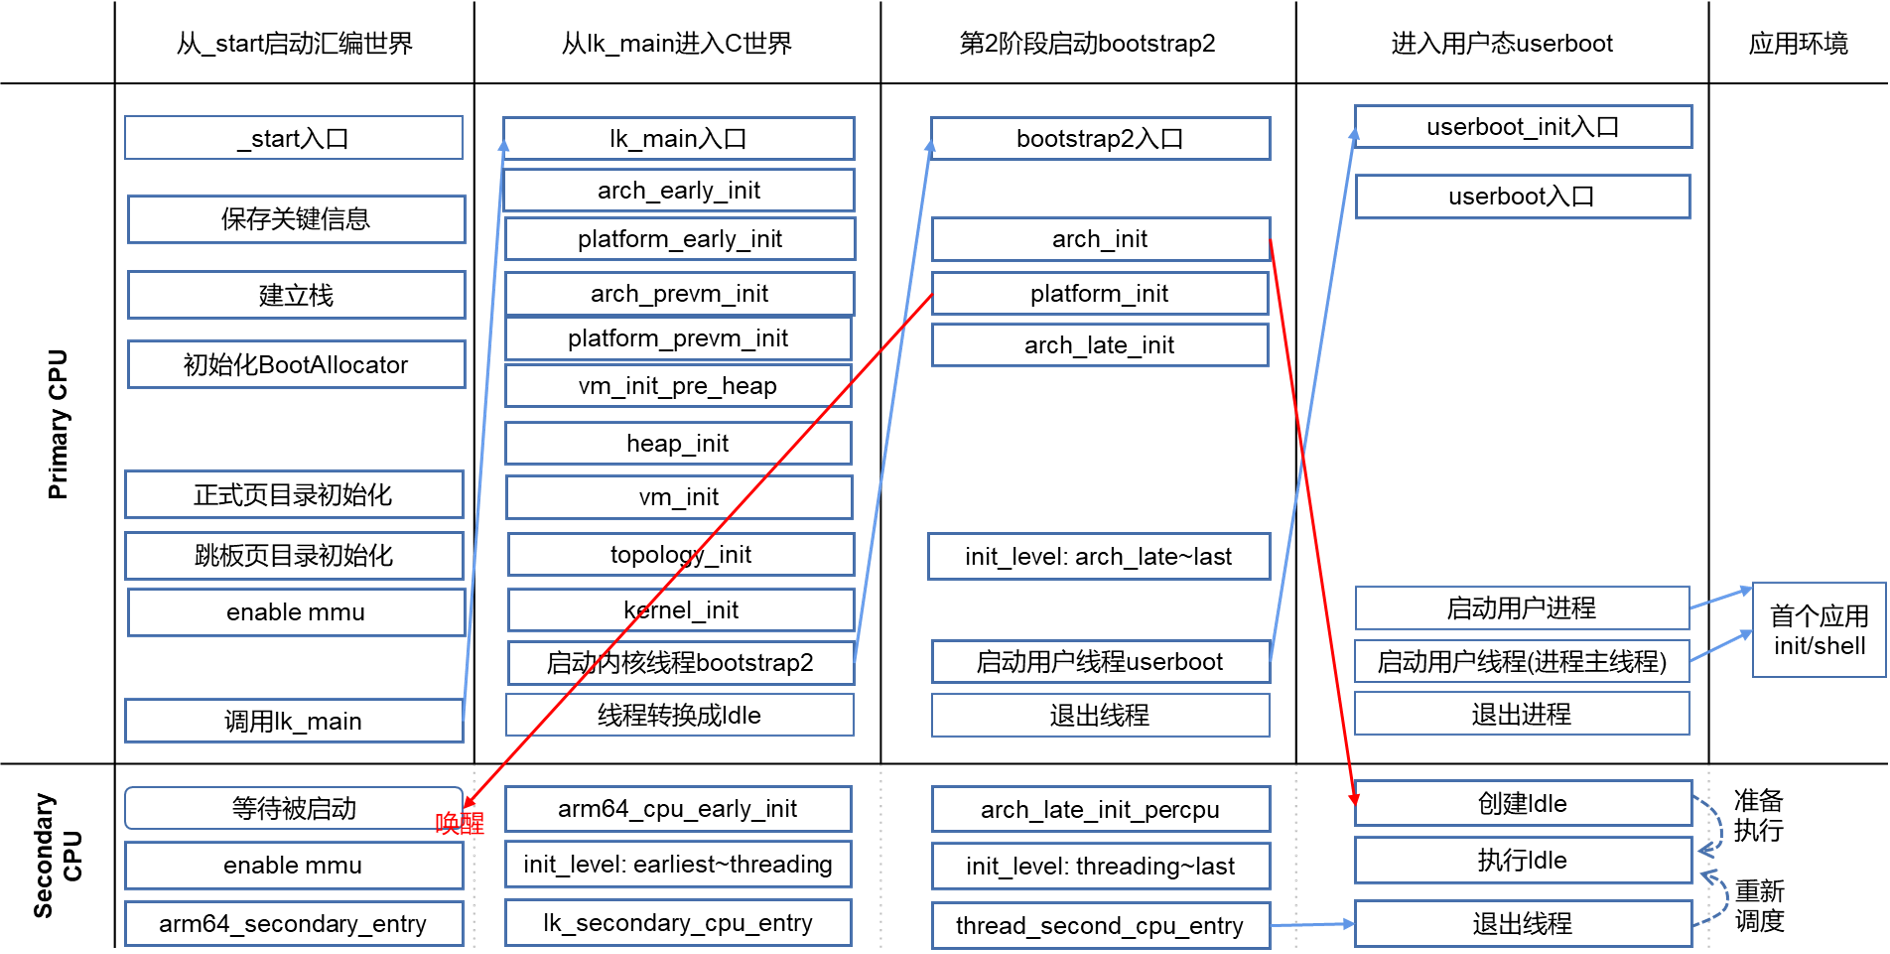
\includegraphics[width=1.0\linewidth]{zircon_flow.png}
			\caption{Zircon总体流程图}
		\end{figure}
	\end{frame}

	\subsection{入口\_start}

	\begin{frame}
		\frametitle{1 入口\_start【kernel/arch/arm64/start.S】}
		\begin{enumerate}
			\item 根据cpuid判断当前cpu身份,0是primary cpu,其它是secondary
			\item primary cpu负责启动工作,所以需要保存引导信息,包括:\\
			handoff地址:上一阶段bootloader传递参数和数据块的开始地址;
			内核入口\_start地址:kernel image的物理地址;
			EL模式:Arm CPU运行级别;
			\item 记录第一条指令的ticks计数作为时间戳\\
			Zircon在各处设置时间戳,度量关键阶段的启动时间。
			\begin{block}{}
				在riscv ISA,我们通过SBI\_PMU\_HW\_CPU\_CYCLES实现。
			\end{block}
			\item 确保当前EL是1,即OS级别,否则切换到OS级
			\begin{block}{}
				zCore也应该检查一下是否S模式,如果意外当前是M模式,要定一个处置策略。
			\end{block}
			\item 启用icache和dcache:Riscv ISA不涉及
			\item 把secondary cpus送去等待,等待primary cpu完成初始化再唤醒它们
			\item 清零BSS
			\item 为primary cpu设置内核栈,该栈在BBS段,长度两个页面
			\begin{block}{}
				如前面提到,zCore仿照该方式,预先只为primary准备栈,后面再按照CPU总数量,按需分配栈
			\end{block}
		\end{enumerate}
	\end{frame}

	\begin{frame}
		\frametitle{1 入口\_start【kernel/arch/arm64/start.S】}
		\begin{enumerate}\setcounter{enumi}{8}
			\item 初始化早期内存分配器boot allocator\\
			两个成员start和end标记已分配区域的开始和结束地址。
			目前还没有分配,所以start/end都设置成kernel image的结束地址\_end,这个也是传统上堆的开始处。
			\item 初始化根页目录,在虚拟地址空间中线性偏移映射两个地址区间
			\item 整个物理地址空间映射到虚拟地址空间的固定位置\\
			参数KERNEL\_ASPACE\_BASE指定虚拟空间位置, ARCH\_PHYSMAP\_SIZE指定被映射的物理空间范围。
            在Arm64 ISA,ARCH\_PHYSMAP\_SIZE是512G,所以实质上是整个物理空间。
			映射区域标识为MMU\_PTE\_KERNEL\_DATA\_FLAGS,即只允许读写。
			\item 内核本身占据的物理空间映射到虚拟地址空间的固定位置(由参数KERNEL\_BASE决定)\\
			映射区域标识为MMU\_PTE\_KERNEL\_RWX\_FLAGS,因为包含代码和数据,所以允许读写执行。
		\end{enumerate}
	\end{frame}

	\begin{frame}
		\frametitle{1 入口\_start【kernel/arch/arm64/start.S】}
		\begin{enumerate}\setcounter{enumi}{8}
			\item 由此在Boot阶段将形成如下的映射布局。内核image在虚拟空间中会被同时映射到两个区间,但是访问权限不同。
			\begin{figure}
				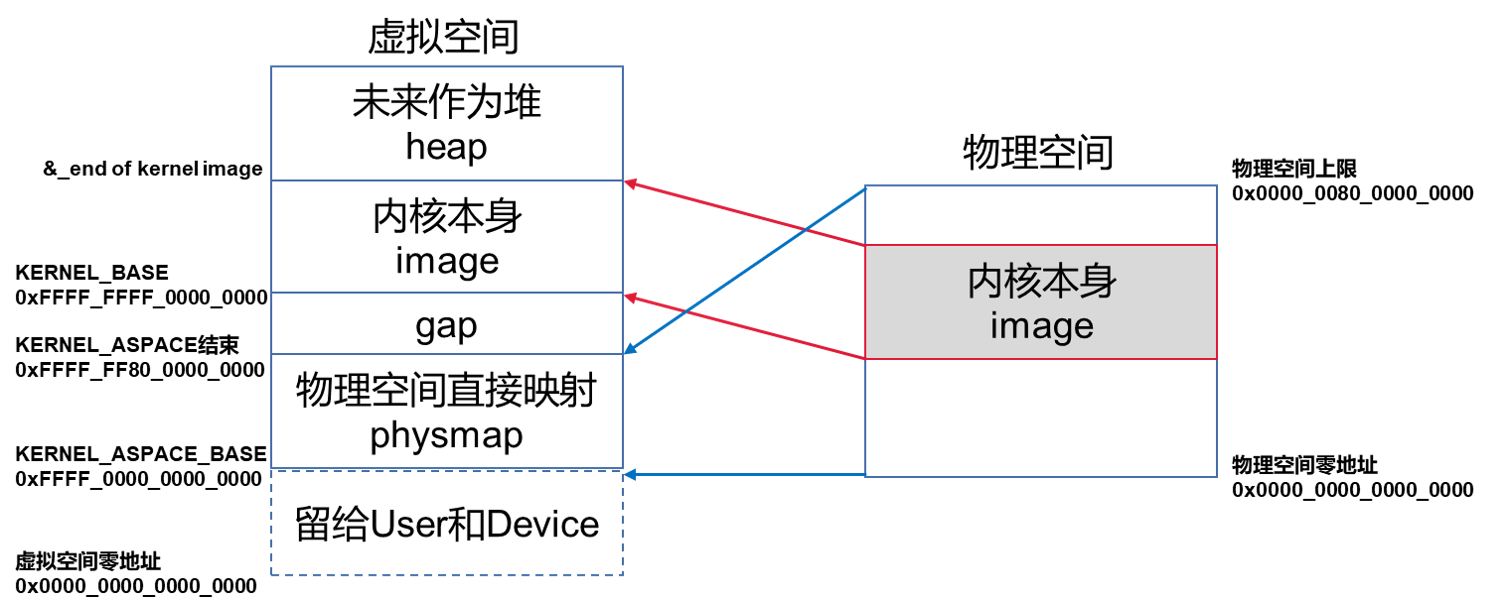
\includegraphics[width=0.6\linewidth]{zircon_aspace.png}
				\caption{Zircon空间映射布局}
			\end{figure}

			\begin{block}{}
				可以借鉴zircon这个办法:规划时先定分页模式(默认4级页表,相当于RISCV的SV48) ,再根据模式定参数(KERNEL\_BASE和KERNEL\_ASPACE\_BASE),划分出各区域;
				实现中通过kernel vmar管理该布局。
			\end{block}
		\end{enumerate}
	\end{frame}

	\begin{frame}
		\frametitle{1 入口\_start【kernel/arch/arm64/start.S】}
		\begin{enumerate}\setcounter{enumi}{10}
			\item 准备跳板 页根目录,准备启用paging。这个机制与zCore目前一致。
			\item 启用paging\\
			Prmiary hart本身跳转到虚拟空间;然后通知secondary harts,跳板准备完毕,所有secondary harts启用分页后,又会进入spin状态,等待下一个唤醒信号。
			\item 由于空间的切换,内核栈必须重置。\\
			设置线程指针寄存器tpidr\_el1:当前的执行流相当于第一个kthread,zircon定义了一个线程对象表示它,然后把指针存到寄存器tpidr\_el1 。
			将来运行过程中,主要通过这个指针寄存器的切换实现任务的切换。Linux kernel for RISCV也有对应的实现机制:
			寄存器TP在启动阶段指向idle task,TP始终指向当前任务,切换任务时切换TP。
			设置percpu管理数组:现在只需要为Primary Hart设置,对应于percpu的0号元素。
			\item 再次采样计数器ticks,减去开始时的ticks,度量第一阶段的启动速度。
			\item 准备跳转lk\_main,进入C世界\\
			以上只是primary cpu的执行流程,对于arm64,开始只有一个ID为0的cpu作为primary启动,随后必须由它去启动其它cpus。
		\end{enumerate}
	\end{frame}

	\subsection{C入口lk\_main}

	\begin{frame}
		\frametitle{2 C入口lk\_main}
		\begin{enumerate}
			\item 初始化线程上下文\\
			初始化线程链表
			初始化percpu的boot\_cpu信息
			构造本cpu的idle线程,加入线程列表,idle作为cpu的保底调度线程
			\item 早期日志初始化
			\item 动态Hook:从Earliest ~ Arch\_early\\
			只有一个Hook,init\_build\_id用于生成版本和编译ID
			\item 体系结构早期初始化:Arch\_early\_init\\
			(1)Cpu早期初始化
			(2)Percpu早期初始化
			(3)设置异常向量入口
			(4)保存cpu features
			(5)启用中断
			(6)MMU早期初始化:初始化ASID分配器
			\item 动态Hook:从Arch\_early ~ Platform\_early
			\item 保存handoff地址,这个是上阶段bootloader传递数据的入口
			\item 平台早期初始化:platform\_early\_init\\
			(1)设置一个系统保留内存区域的链表rev\_list,按照地址从小到大排列。
			先把kernel image本身占据的区间加入rev\_list。\\
			(2)从PhysHandoff发现所有的内存区域,分别处理
			\begin{block}{}
				zCore中,我们通过解析DTB,执行同样的逻辑。
			\end{block}
		\end{enumerate}
	\end{frame}

	\begin{frame}
		\frametitle{2 C入口lk\_main}
		\begin{enumerate}\setcounter{enumi}{8}
			\item 处理NVRAM:该区域主要用作crashlog和tracelog,加入rev\_list。
			\item 处理Common内存区域。包括三类:RAM/Peripheral/Reserve。
			\item 处理RAM:加入mem\_arena数组,上限16个。\\
			Zircon对物理内存的概念是三级:Node、Arena和Page。
			Node可以由一至多个Arena构成,每个Arena内部地址是连续的,内部特性是一致的。
			每个Arena在自己管理区域的顶端位置,设置一个page\_array\_数组,每元素对应维护本区域的页面属性。
			\begin{block}{}
				zCore目标平台采取NUMA的可能性不大,可忽略Node;但是仍可能存在多个Arena,所以保留mem\_arena数组,上限数量16应该是充足的。
			\end{block}
			\begin{figure}
				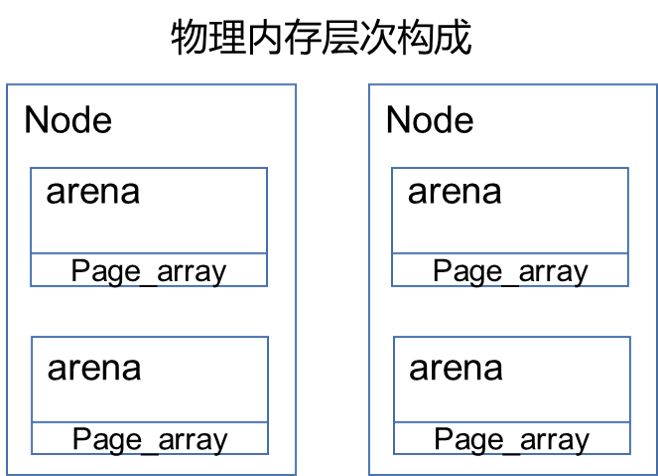
\includegraphics[width=0.3\linewidth]{zircon_pmm.png}
				\caption{Zircon物理内存管理概念}
			\end{figure}
		\end{enumerate}
	\end{frame}

	\begin{frame}
		\frametitle{2 C入口lk\_main}
		\begin{enumerate}\setcounter{enumi}{8}
			\item Peripheral:
            \begin{columns}[c]
                \begin{column}{0.5\textwidth}
                    \begin{center}
                        映射到Kernel image之前的区域中, \\
                        即KERNEL\_BASE之前。上限4个。
                    \end{center}
                \end{column}
                \begin{column}{0.45\textwidth}
                    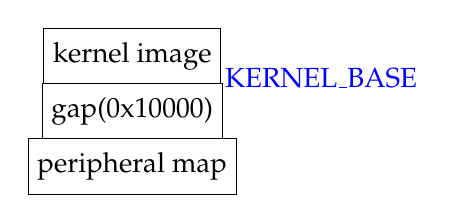
\begin{tikzpicture}
                        \node[rectangle, draw, minimum height=20pt, minimum width=64pt]
                            (1) at (0pt,0pt) {kernel image};
                        \node[rectangle, draw, minimum height=20pt, minimum width=64pt]
                            (2) at (0pt,-20pt) {gap(0x10000)};
                        \node[rectangle, draw, minimum height=20pt, minimum width=64pt]
                            (3) at (0pt,-40pt) {peripheral map};
                        \draw (30pt,-8pt) coordinate node[right, text=blue] {KERNEL\_BASE};
                    \end{tikzpicture}
                \end{column}
            \end{columns}
			\item Reserve:其它系统保留用途的内存区域,加入rev\_list。
			\item 解析命令行,处理针对debuglog和串口的参数。
			\begin{block}{}
				解析dtb获得这些参数, chosen.bootargs对应命令行, chosen.stdout-path对应默认输出设备, \\
                进而解析对应uart设备的参数。
			\end{block}
            \item 查看是否需要执行物理内存扫描检查。\\
            通常的检查方法:向内存单元写入该单元地址, 再读出, 检查一致性。\\
            可以表示为: *addr = addr;
			\item 把ram disk占据区间加入rev\_list\\
            对于arm64, ZBI占用的物理内存空间即ram disk
			\item 如果memory limit存在,对所有的arena区域执行limit交集处理。
			\item 对所有的arena区域与rev\_list执行交集检查,裁剪排除被保留的部分。
			\item 所有保留区域的Page设置为wired,表示被系统保留
		\end{enumerate}
	\end{frame}

	\begin{frame}
		\frametitle{2 C入口lk\_main}
		\begin{enumerate}\setcounter{enumi}{8}
			\item 系统驱动初始化: 包括Uart、gic、watchdog、timer、psci, power\\
            初始化过程利用了C++的std::visit模式, 形式是visit(lambda, variant), \\
            根据variant的具体类型, 调用相应的处理函数。以Uart为例, serial(variant)的类型是UartDriver,\\
            这是抽象类型; 各种实际的串口驱动在DriverBase的帮助下,实现UartDriver并定义方法, \\
            例如: ns8250(定义在system/ulib/uart/include/lib/uart/ns8250.h)就是实际的串口驱动。\\
            默认情况下, serial是null驱动; 实际驱动将会在系统启动早期, 注册到serial, 此后可以被visit访问。
			\item 动态Hook:从Platform\_early ~ Arch\_prevm。初始化timer和全局随机数种子发生器。
			\item 虚拟内存初始化准备(体系结构相关):arch\_prevm\_init
			\item 动态Hook:从Arch\_prevm ~platform\_prevm
			\item 虚拟内存初始化准备(平台相关):platform\_prevm\_init\\
			(1)内核空间惯例初始化:以根vmar为树根的树形管理,每一个结点代表位于父节点区间内的子区间
			(2)初始化physmap vmar:对应于前面布局中的physmap区域
			\item 动态Hook:从platform\_prevm ~ vm\_preheap
		\end{enumerate}
	\end{frame}

	\begin{frame}
		\frametitle{2 C入口lk\_main}
		\begin{enumerate}\setcounter{enumi}{8}
			\item 堆初始化前准备vm\_init\_preheap\\
			(1)内存地址空间初始化\\
			建立vmar的树表示kernel aspace\\
			root\_vmar树根下,建立三个子vmar(对应前面的虚拟内存布局):\\
			Vmar\_physmap:物理内存空间直接映射(按照512G,可认为就是全部物理内存空间)\\
			Vmar\_image:内核image 自身占据区域\\
			Vmar\_heap:从\&\_end开始的堆区域\\
			(2)Vmar正式加入树(Activate vmar):\\
			前置检查vmar在parent的范围内,且与当前所有的兄弟不冲突。\\
			(3)分配vmar:在parent区间中寻找一块未使用的和符合对齐要求的区间\\
			(4)遍历boot allocator,把目前已经分配出去Page标记为wired进行保留\\
			(5)分配一页作为只读的Zero Page,供整个系统使用\\
			(6)匿名页面请求器初始化
			\item 动态Hook:从vm\_preheap ~ heap:仅一个HOOK,初始化内存越界检查机制asan
			\item 初始化堆heap\_init\\
			(1)初始化分配器cmpct,每次heap\_grow增加256K空间\\
			(2)扩展堆heap\_grow:优先使用缓存,没有缓存时从pmm申请\\
			Cmpct相当于Linux kernel的buddy system;\\
            Pmm的Node和Area对应于pgdat和zone
		\end{enumerate}
	\end{frame}

	\begin{frame}
		\frametitle{2 C入口lk\_main}
		\begin{enumerate}\setcounter{enumi}{10}
			\item VirtualAllocat基于堆实现\\
			(1)通过BitmapAlloc从位图中查找并标记分配\\
			(2)从cmpct中申请物理Page\\
			(3)把物理Page映射到虚拟空间,返回地址
			\item 动态Hook:heap ~ vm,包括如下几个hook
			\item 资源系统初始化Hook\\
			mmio资源:64位空间for mmio\\
			中断资源:全局中断控制器gic,irq资源\\
			系统资源:ioport,root,smc,system,count
			\item Version打印Hook
			\item 控制台初始化Hook:即对Console参数的处理和分配缓冲区
			\item 虚拟内存初始化vm\_init
			\item 地址空间空隙保护\\
			physmap虚拟空间中可能存在gap区域,对它们设置特殊属性,禁止访问
			\item 对所有直接映射的Arenas区域进行保护:所有的Arena区域都不可执行
			\item 针对内核image各段(代码段、数据段)的特性进行保护
			\item 对vmar\_physmap执行保护策略
			\item 设置threshold(即水位),当前可分配空间低于该界限时自动从pmm填充
		\end{enumerate}
	\end{frame}

	\begin{frame}
		\frametitle{2 C入口lk\_main}
		\begin{enumerate}\setcounter{enumi}{20}
			\item 动态Hook:vm ~ topology\\
			(1)从Handoff解析topology信息,填充管理cpu的层次结构\\
			如果zCore目标平台不涉及NUMA,只要初始化一个cpu管理数组\\
			(2)如果存在periph vmar,对其设置保护策略\\
			\item NUMA初始化:略过
			\item 动态Hook:topology ~ kernel
			\item 内核初始化:kernel\_init
			\item 动态Hook:kernel ~ threading\\
			(1)初始化pmm前端页面缓存\\
			为每个cpu设置一定数量的Pages作为缓存,避免每次都要从pmm中申请\\
			(2)缓冲区链初始化buffer\_chain\_cache\_init\\
			Zircon的buffer类似于linux kernel的buffer,可以跨多个Page,但是它们主要的服务对象是通道对象Channel。所以这个链的作用相当于Slab for channel。\\
			(3)端口缓冲区初始化port\_observer\_cache\_init\\
			为端口的observer和packet的分配提供缓冲页面,相当于Slab for port。\\
			(4)代码覆盖率检测机制初始化InitSancov\\
			(5)写时拷贝缓冲区初始化InitCowPages:预留一部分Pages专用于该目的\\
			(6)初始化Percpu数组\\
			每个cpu按照逻辑ID在percpu数组中对应一个管理对象,其中0号时Primary cpu。\\
			启动早期已经初始化Primary cpu,现在完成其它secondary cpus。
			\item 启动bootstrap2线程,在线程中开启下一阶段的启动\\
			创建启动线程见3;bootstrap2的执行逻辑见4。
		\end{enumerate}
	\end{frame}

	\subsection{启动内核线程,准备第二阶段启动}

	\begin{frame}
		\frametitle{3 启动内核线程,准备第二阶段启动}
		\begin{enumerate}
			\item 线程结构Thread\\
			(1)调度器scheduler\_state:调度相关,例如优先级\\
			(2)等待队列wait\_queue\_state:在等待队列中的接入点\\
			(3)任务task\_state:任务相关,记录执行入口entry和启动参数arg\\
			(4)抢占preemption\_state:抢占相关\\
			\item 创建线程实例CreateEtc\\
			(1)分配一个线程实例\\
			(2)在task\_state中记录entry 和 arg\\
			(3)通过调度器初始化该线程,作用在scheduler\_state上\\
			(4)设置线程栈\\
			(4.1)从内核空间的root\_vmar中分配子vmar,大小根据本体系结构的默认栈大小值\\
			(4.2)分配COW页面,返回封装它们的VMO对象\\
			(4.3) 为VMO对象在虚拟空间建立映射,然后触发fault in,完成内容的填充\\
			(4.4)根据体系结构的要求,初始化栈帧\\
			(4.5)把线程推入thread list\\
			\item 脱离父线程Detach
			标记本线程detached
			\item 恢复(或启动)线程\\
			主要通过Scheduler::Unblock解除线程的阻塞状态,实现恢复或者启动\\
			(1)取时间戳\\
			(2)取目标CPU,然后根据cpu逻辑号找到对应的scheduler实例\\
			(3)设置线程状态为ready,推入scheduler的调度队列\\
			(4)请求reschedule,促使该线程被调度到
		\end{enumerate}
	\end{frame}

	\subsection{在内核线程中,执行第二阶段启动}

	\begin{frame}
		\frametitle{4 第二阶段启动bootstrap2(在内核线程中执行)}
		\begin{enumerate}
			\item 设置当前线程的CPU亲和性(绑定primary cpu)\\
			当前线性继续代表Primary CPU执行初始化,因此必须绑定在primary cpu上。
			\item 动态Hook:Threading ~ Arch
			\item 对象初始化Hook\\
			(1)为Handle准备存储区域:分配一部分Pages作为作为分配handle的缓存\\
			(2)初始化Executor:系统调用与底层内核资源的中间层\\
			(3)创建root\_job以及它的Handle
			\item 全局随机数发生器Hook:建立并保证线程安全
			\item 死锁检测
			\item 定时器初始化:启用时钟中断,设置时钟stream模式
			\item DPC初始化:Deffered Procedure Calls\\
			每个cpu的percpu维护一个DPC队列,保存延迟调用的任务。
			通常用于减轻中断处理的任务,从中断上下文转到普通上下文中处理。
			\item 体系结构初始化arch\_init
			\item 初始化percpu关于中断的部分,然后让本cpu上线,并启用IPI中断
			\item 为每个secondary cpu创建IDLE Thread(Primary 的之前已经建立)
			\item 动态Hook:Arch ~ Platform
			\item 性能监控Hook:perfmon\_init
		\end{enumerate}
	\end{frame}

	\begin{frame}
		\frametitle{4 第二阶段启动bootstrap2(在内核线程中执行)}
		\begin{enumerate}
			\item 初始化debug端口Hook:Debug Port用于从外部连接和调试Soc
			\item 平台初始化platform\_init
			\item 注册CPU逻辑ID与物理ID的映射表
			\item 为所有secondary cpu准备内核栈
			\item 唤醒启动所有的secondary cpus
			\item 启动一个线程,用于检查是否所有的cpu都已经成功启动\\
			具体实现方法:等待mp\_state.online\_cpus位图的所有有效位都已经置一 (每个CPU启动成功后会在对应位上置一)
			\item 内核驱动后期初始化:\\
			(1)Uart的后期初始化\\
			(2)Gic、hdmi、rng、watchdog后期初始化
			\item 动态Hook:Platform ~ Arch\_late\\
			(1)调试日志hook:启动debuglog线程\\
			(2)全局随机数发生器Hook:生成种子\\
			(3)时间段度量机制初始化\\
			(4)所有cpu启动计数
		\end{enumerate}
	\end{frame}

	\begin{frame}
		\frametitle{4 第二阶段启动bootstrap2(在内核线程中执行)}
		\begin{enumerate}
			\item 体系结构后期初始化Arch\_late\_init\\
			标记当上下文切换时,分支预测器是否需要刷新
			\item 动态Hook:Arch\_late ~ Last:\\
			现在仅有一个Hook:User\\
			(1)显式内核启动后空闲的页面数量\\
			(2)初始化计数器,记录zircon 从启动开始到完成的总时间。\\
			(3)初始化Shell:启动主控台\\
			(4)初始化资源过滤器:对资源进行保护\\
			目前把RAM加入过滤器,不允许userspace直接访问;但是允许直接访问reserve的RAM区域,因为有可能用户进程在其中有mmio区间。\\
			(5)初始化Trace:ktrace\_init\\
			(6)启动线程处理全局随机数发生器\\
			(7)用户态初始化userboot\_init\\
			以下开启下一阶段,将从内核态转入用户态。流程概述\\
			(7.1)Userboot\_init先做准备工作(详见5) ,最后启动一个线程做后续工作\\
			(7.2)在线程中,通过vdso启动第一个用户态程序UserBoot(详见6)\\
			(7.3)UserBoot依然是系统的一部分,它负责启动第一个真正有用的用户程序(zCore目前就是sh)
		\end{enumerate}
	\end{frame}

	\subsection{准备启动用户态程序userboot\_init}

	\begin{frame}
		\frametitle{5 准备启动用户态程序userboot\_init}
		\begin{enumerate}
			\item 构造消息包packet,作为句柄数组的载体,该消息将来会通过通道channel传给进程
			\item 通过工厂ProcessDispatcher来创建进程process\\
			(1)在root\_job下构建一个process\\
			(2)创建process工厂的句柄\\
			(3)创建vmar工厂的句柄\\
			(4)返回上述句柄
			\item 创建进程对象process和地址区间对象vmar的句柄,填充到句柄数组中
			\item 分配资源句柄,填充到句柄数组中\\
			主要资源包括root, mmio, irq, smc, system以及root\_job,这些资源的句柄将被传递给process供它使用。
			\item 创建和获取各vdso和vmo对象\\
			vDSO都是ELF格式的对象,类似于DSO。\\
			区别是vDSO是kernel直接在地址空间中分配并填充构成的。\\
			(1)通过申请空间和初始化vDSO基础结构\\
			(2)创建常量,填充到vDSO\\
			(3)Patch vDSO,加入必要的系统调用\\
			(4)通过bootstrap\_vmos,获取各种参数填充vDSO\\
			(5)把vDSO的句柄和ZBI的句柄都填充到句柄数组
		\end{enumerate}
	\end{frame}

	\begin{frame}
		\frametitle{5 准备启动用户态程序userboot\_init}
		\begin{enumerate}
			\item 构造channel,包括两端,内核端和进程端\\
			(1)通过channel的内核端,把前面创建的消息写入channel\\
			(2)channel用户端会在process启动时交给它\\
			进程一旦启动,就能够从channel中读消息,取出句柄数组
			\item 把userboot\_image映射到vmar管理的空间中\\
			(1)Image包含userboot本身和紧跟的vdso,它们作为进程root\_vmar的子vmar被分别映射到虚拟空间\\
			(2)返回两个关键信息,userboot的执行入口entry和vdso\_base地址\\
			\item 映射栈
			\item 创建用户进程中的首个线程\\
			类似于Process,通过ThreadDispatcher,即线程工厂创建线程。\\
			但是该线程的启动比较特殊,在切换运行状态的同时,完成线程启动。\\
			(1)伪造栈帧现场,做好返回用户态的准备\\
			关键是两个参数:线程entry作为epc,线程栈作为ustack pointer。\\
			(2)处理待决信号(pending signal):这里正是处理信号的时机\\
			(3)切换到用户态arch\_enter\_uspace(iframe)\\
			禁止中断,基于前面伪造的返回现场,通过eret指令返回用户态执行entry,此后就是在userspace执行逻辑。
			\item 已经完成从内核态到用户态的切换,执行第一个用户态程序UserBoot(详见6)
		\end{enumerate}
	\end{frame}

	\subsection{第一个用户态程序userboot}

	\begin{frame}
		\frametitle{6 第一个用户态程序userboot}
		\begin{enumerate}
			\item 入口\_start(zx\_handle\_t arg)\\
			arg参数就是由内核创建的channel的用户端
			\item 从channel读出消息,取出所有句柄
			\item 通过对应句柄,获取vmar对象和process对象
			\item 通过句柄从ZBI中取得bootfs,这是一个简单的文件系统
			\item 从ZBI中取得命令行参数
			\item 加载真正的用户态进程(init/sh等),移交执行权,此刻系统启动阶段完成
			\item 本进程正常退出zx\_process\_exit(0)
		\end{enumerate}
	\end{frame}

	\subsection{Secondary CPUs初始化与启动过程总结}

	\begin{frame}
		\frametitle{7 Secondary CPUs初始化与启动过程总结}
		\begin{enumerate}
			\item 确保在E1态运行
			\item 启用icache/dcache/ucache
			\item 取得跳板页目录地址和正式根目录地址
			\item 等待prime的通知,启用mmu分页
			\item 等待secondary boot信号,开始正式运行
			\item 设置栈\\
			(1) primary cpu在发出secondary boot信号前,按照cpu总数为其它所有的cpu准备好栈空间(地址连续)\\
			(2) 这里secondary cpu根据自己的逻辑ID定位对应的栈\\
			\item 进入secondary入口执行arm64\_secondary\_entry\\
			(1)初始化percpu结构\\
			(2)设置本cpu异常入口\\
			(3)获取本cpu features\\
			(4)启用中断\\
			(5)等待secondaries\_released信号\\
			该信号在primary\_cpu在arch\_init中为所有secondary cpus创建IDLE thread之后。
			\item 构造Thread,继续执行初始化任务
		\end{enumerate}
	\end{frame}

	\begin{frame}
		\frametitle{7 Secondary CPUs初始化与启动过程总结}
		\begin{enumerate}
			\item 执行动态hook,从Earliest ~ Threading\\
			注意:各种hook在注册时,指定了适用的目标。\\
			大多数HOOK的标识是LK\_INIT\_FLAG\_PRIMARY\_CPU,即只对primary cpu有效。\\
			只有少数标记为LK\_INIT\_FLAG\_SECONDARY\_CPUS或LK\_INIT\_FLAG\_ALL\_CPUS的Hook会在这被执行。
			\item 初始化cpu的根中断管理器
			\item 进入线程执行最后阶段的初始化\\
			(1)Percpu的后期初始化:针对体系结构的特殊要求\\
			(2)动态Hook:Threading~Last\\
			(3)死锁检测
			\item secondary cpu执行初始化任务的线程退出\\
			(1)从调度器中删除本线程\\
			(2)执行Thread::Current::Exit()退出\\
			(2.1)标记本线程状态death\\
			(2.2)设置返回码\\
			(2.3)清理资源\\
			如果是标记了Detached的线程,自己清理资源,然后直接从全局线程list中删除;\\
			否则需要通知parent thread清理资源(Parent正在阻塞等待本线程退出)。\\
			(2.4)执行重调度RescheduleInternal,切换到其它线程\\
			Secondary cpu在启动阶段,没有其它的线程或进程在执行,所以退回到本cpu的IDLE Thread。
		\end{enumerate}
	\end{frame}

	\subsection{Prime CPU成为IDLE}

	\begin{frame}
		\frametitle{8 Prime CPU成为IDLE}
		\begin{enumerate}
			\item 设置名称“idle [cpuid]”
			\item 标记本线程是IDLE
			\item 从调度器中删除,不参与调度,idle就是垫底的
			\item 线程设置running状态
			\item 设置当前CPU是active状态,表示活动中
			\item 设置pending for preemption状态,确保重调度reschedule可以执行
			\item 启用preempt抢占机制
			\item 启用本CPU的中断
			\item 进入无限循环等待状态
		\end{enumerate}
	\end{frame}

	\section{对zCore组织研究开发的建议}

	\begin{frame}
		\begin{center}
			{\LARGE 对zCore组织研究开发的建议\\}
		\end{center}
	\end{frame}

	\subsection{zCore项目结构调整建议}

	\begin{frame}
		\frametitle{zCore项目结构调整建议}
		\begin{enumerate}
			\item 建议分别设立arch与platform两种目录\\
			Zircon对这两种目录是区别对待的: \\
			(1)arch:对应体系结构,包含arm64和x86。这里面处理是特定于cpu指令架构的东西。\\
			(2)platform: 对应于平台,涉及总线及外设标准。包括两类:\\
			(2.1)generic-arm是对应终端、嵌入式设备等soc平台;\\
            (2.2)pc对应的是传统的个人电脑或工作站。\\
			arch和platform两个维度可以正交,搭配出不同的组合。
			例如,同一种arch可以配套不同的platform,而同一种platform也可以搭配不同的arch。
			\item 建议取消kernel-hal\\
			zCore当前源码中,条件编译的地方是比较多的,似乎kernel-hal并未起到很好的隔离作用,而且采用这种方式把代码隔成两块,在阅读维护代码时感觉不太顺畅。
			建议借鉴zircon的处理方式:
			参照上一条的建议,把kernel-hal的代码以及zCore主项目中条件编译的代码区分一下,分别安排到arch和platform目录下。
			参照zircon在初始化阶段建立静态和动态hook机制,把arch和platform目录下的代码转换为实现对应阶段的静态hook或注册为动态hook。
			\item 建议把libos放到platform下面,作为一种特殊的平台处理
		\end{enumerate}
	\end{frame}

	\subsection{基于开源社区组织zCore研发的建议}

	\begin{frame}
		\frametitle{基于开源社区组织zCore研发的建议}
		\begin{enumerate}
			\item 目的:\\
			通过开源的方式组织安全操作系统的研究和开发,打开从底层硬件到上层应用各层次专业人员协作参与的通道,
			打开各种应用环境下和测试环境下用户反馈的通道,形成持续改进的闭环。
			\begin{figure}
				
\includegraphics[width=1.0\linewidth]{open_community.png}
			\end{figure}
			\item 组织:\\
			初期两级构成:一级维护者+贡献者。维护者不少于3人,在实际的社区运行中,逐渐形成维护者团队。
			\item 设施:\\
			开发协作主要基于传统的开发者邮件列表(maillist),这个应该比较符合多数系统软件开发者的习惯。
			接受用户反馈可以选择采用论坛或邮件列表的方式,维护者轮班负责收集归纳反馈和回复有代表性的用户问题。
			\item 机制:\\
			(1)审核机制:两个reviewed-by过关;\\
			(2)发版机制:三个月一个版本,其中两个月开放期,一个月封闭测试期。
		\end{enumerate}
	\end{frame}

	\subsection{基于zCore可能展开的研究方向的建议}

	\begin{frame}
		\frametitle{基于zCore可能展开的研究方向的建议}
		\begin{enumerate}
			\item RUST语言对系统级开发的支持\\
			总结在基于rust研发zCore过程中的经验,研究并提出rust改进方案,参与rust社区在支持系统级开发方面的工作。
			\item 基于RISCV体系结构的软硬件协同设计\\
			RISCV作为一种开放式的体系架构,支持对其进行非标准扩展。
			根据zCore的目标,重点针对安全性和关键性能方面,研究软硬件协同的设计方案,研究通过扩展ISA和硬件辅助提升安全性和性能的关键技术与实现。
			\item 线程+异步混合调度机制\\
			线程和异步各有自身特点和适用场景,不是替代关系。研究zCore同时支持这两种机制的方案。
			\item “元编程”在系统级开发中的应用
			基于zCore开发的实践,研究通过Rust语言的宏在高抽象层次表述对象的方法,研究形式化方法在系统设计和验证中的的应用。减少冗余代码,提高一致性和开发者的开发效率。
		\end{enumerate}
	\end{frame}

	\subsection{对zCore研发里程碑的补充建议}

	\begin{frame}
		\frametitle{对zCore研发里程碑的补充建议}

		\begin{table}\resizebox{\linewidth}{!}{
			\begin{tabular}{l l l l}
				\toprule[2pt]
				\textbf{2023 架构设计} & \textbf{2025 基本实现} & \textbf{2026 示范应用} & \textbf{2030 推广生态}\\
				\midrule[1pt]
				{创新操作系统架构} & {软硬件协同设计} & {突破卡脖子技术} & {操作系统全链突破} \\
				\hline
				\makecell[l]{\\提出基于Rust的异步可扩\\展操作系统架构,较现有\\OS提供更多层次的软件并行\\性表达能力,为构建自主\\可控IT生态奠定OS基础。\\} &
				\makecell[l]{研制适配的无人系统/机器人\\的编程、编译与运行时系统,\\解决新型OS下的软件开发和\\运行问题。} &
				\makecell[l]{OS可运行在主流处理器\\和新型处理器原型之上,\\移植典型示范应用,\\解决操作系统系统纵横向\\整合的生态问题。} &
				\makecell[l]{研制成功安全高性能新型\\操作系统,并在实际产业\\中大规模使用,形成围绕\\操作系统的新产业生态。} \\
				\hline
				\makecell[l]{\\1 以RISCV为主平台,参照\\zircon的架构实现,调整完善\\zCore。\\
							 2 开源社区的机制与设施建立,\\尝试运行。\\
							 3 研究RUST语言对系统级\\开发的支持。\\
							 4 研究线程+异步混合调度\\机制。} &
				\makecell[l]{\\1 zCore支持Linux和zircon\\两种应用环境,两种系统调用\\接口完备,主流应用的运行\\性能与参照系统持平。\\
							 2 开源社区维护者团队成熟,\\按照模块分工,测试系统完备,\\具备保障持续发版的能力。\\
							 3 研究基于RISCV体系结构\\的软硬件协同设计。} &
				\makecell[l]{1 zCore支持其它主流的体系\\架构,支持各国产化体系架构。\\
							 2 开源社区维护团队形成多级\\结构,吸收各厂商和组织的人员\\作为外围维护者负责相应的\\体系结构模块或功能模块审核。\\
							 3 研究元编程在系统级开发中\\的应用。} &
				\makecell[l]{1 zCore根据AIoT的发展情况,\\面向当时需求旺盛的代表性应用\\场景,在操作系统层面具备良好\\的支持能力和快速改\\进能力。\\
							 2 在操作系统领域,成为国际化\\开源社区。} \\
				\bottomrule
			\end{tabular}
			}
			\caption{zCore研发里程碑}
		\end{table}
	\end{frame}

	\begin{frame}[plain]
		\begin{center}
			{\Huge The End}

			\bigskip\bigskip % Vertical whitespace

			{\LARGE 请老师们批评指正!}
		\end{center}
	\end{frame}

\end{document}